This section analyzes the performance of different neural network configurations applied to the Lorenz system. All data in this section is generated using the following settings:
\begin{itemize}
    \item \textbf{BDF Scheme} (Backward Differentiation Formula)
    \item \textbf{M = 3}: Order of the BDF scheme
    \item \textbf{Skip = 1}: Time step interval used between evaluations
    \item \textbf{Number of iterations = 50,000}: Maximum training iterations
    \item \textbf{Initial Position}: The trajectory calculations start from a given initial position in the Lorenz system $x = -8.0, y = 8.0, z = 27$.
    \item \textbf{System parameters}: $\sigma = 10.0$, $\beta = 8.0/3.0$ and $\rho = 28.0$.
\end{itemize}

The experiments involve neural networks with 5 layers and varying neurons per layer (40, 60, 80, and 100). For each configuration, we observe errors along the \( x \), \( y \), and \( z \) axes of the Lorenz attractor, as well as the minimum and last loss values.

\section{Analysis of Neural Network Structure}
\subsection{Error Analysis}

Table \ref{tab:error} shows the errors for each configuration along each axis:

\begin{center}\label{tab:error}
\begin{tabular}{|c|c|c|c|}
\hline
Neurons per Layer & \( \text{Error}_x \) & \( \text{Error}_y \) & \( \text{Error}_z \) \\
\hline
40 & 1.4029 & 1.3886 & 0.4453 \\
60 & 1.2870 & 1.2966 & 0.5114 \\
80 & 1.2897 & 1.3255 & 0.4813 \\
100 & 1.2540 & 1.2523 & 0.4795 \\
\hline
\end{tabular}
\end{center}

\noindent
Errors along the \( x \) and \( y \) axes generally decrease as the number of neurons increases, suggesting that higher neuron counts improve the network’s ability to capture the dynamics along these dimensions. However, the reduction in error becomes less significant beyond 60 neurons, indicating diminishing returns. The error on the \( z \)-axis is lower and stabilizes with configurations of 80 neurons and above, possibly because the \( z \)-dimension is simpler for the model to approximate. In Fig. \ref{fig:trajectory_comparison}, we observe that the model captures the system's behavior effectively. Although the error may seem relatively large, the neural network successfully learns the essential dynamics of the system.

\begin{figure}[h!]
    \centering
    \includegraphics[width=0.8\textwidth]{Images/80x5.png}
    \caption{Comparison of the true and predicted trajectories along the \( x \), \( y \), and \( z \) axes with a $80\text{x}5$ configuration. This illustrates how well this model can capture the behavior of the system.}
    \label{fig:trajectory_comparison}
\end{figure}

\subsection{Loss Analysis}
The minimum and last loss values, representing the lowest and final values of the loss function during training, indicate the network’s convergence behavior and accuracy. 

\begin{center}
\begin{tabular}{|c|c|c|}
\hline
Neurons per Layer & Minimum Loss & Last Loss \\
\hline
40 & 0.0172 & 0.4329 \\
60 & 0.0087 & 0.0151 \\
80 & 0.0063 & 0.0068 \\
100 & 0.0052 & 0.0398 \\
\hline
\end{tabular}
\end{center}

\noindent
The minimum loss consistently decreases with larger networks, showing that higher neuron counts help the network reach lower loss values during training. The last loss value is close to the minimum loss for configurations of 60 and 80 neurons, indicating stable convergence. Interestingly, the 100x5 configuration shows a higher last loss (0.0398), which may suggest overfitting or instability in the training process for networks of this size.

\begin{figure}[h!]
    \centering
    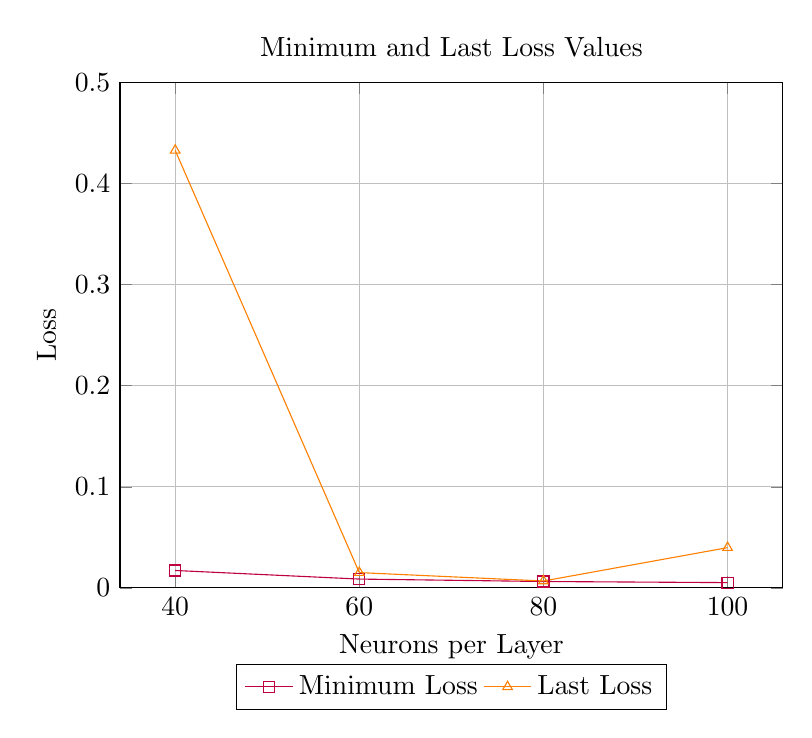
\begin{tikzpicture}
        \begin{axis}[
            width=10cm, height=8cm,
            xlabel={Neurons per Layer},
            ylabel={Loss},
            xtick={40, 60, 80, 100},
            legend style={at={(0.5,-0.15)}, anchor=north, legend columns=-1},
            ymin=0, ymax=0.5,
            grid=both,
            title={Minimum and Last Loss Values}
        ]
        % Minimum Loss
        \addplot[color=purple, mark=square] coordinates {
            (40, 0.0172)
            (60, 0.0087)
            (80, 0.0063)
            (100, 0.0052)
        };
        \addlegendentry{Minimum Loss}

        % Last Loss
        \addplot[color=orange, mark=triangle] coordinates {
            (40, 0.4329)
            (60, 0.0151)
            (80, 0.0068)
            (100, 0.0398)
        };
        \addlegendentry{Last Loss}
        \end{axis}
    \end{tikzpicture}
    \caption{Minimum and last loss values for different network configurations.}
    \label{fig:loss_plot}
\end{figure}

Fig. \ref{fig:loss_plot} illustrates the oscillatory behavior of the loss function during optimization. In this way, After a finite number of iterations, we may reach a local maximum, resulting in a lower optimization level (higher loss), or a minimum, achieving a higher optimization level (lower loss). Setting a minimum error threshold is recommended. However, the solution may still fail to converge, potentially resulting in additional iterations without significant improvement and increased computational expense. 



\section{Analysis of Parameter \( M \)}
This analysis is done using the $80 \times 5$ configuration and varying the value of \( M \) between 1 and 5.


\subsection{Loss Function Analysis Varying \( M \)}

To better illustrate the convergence behavior as \( M \) varies, Figure \ref{fig:loss_M} shows the minimum and last loss values for each \( M \) value. As observed, there is a general trend of decreasing last loss with increasing \( M \), indicating improved model convergence as \( M \) increases.

\begin{figure}[h!]
    \centering
    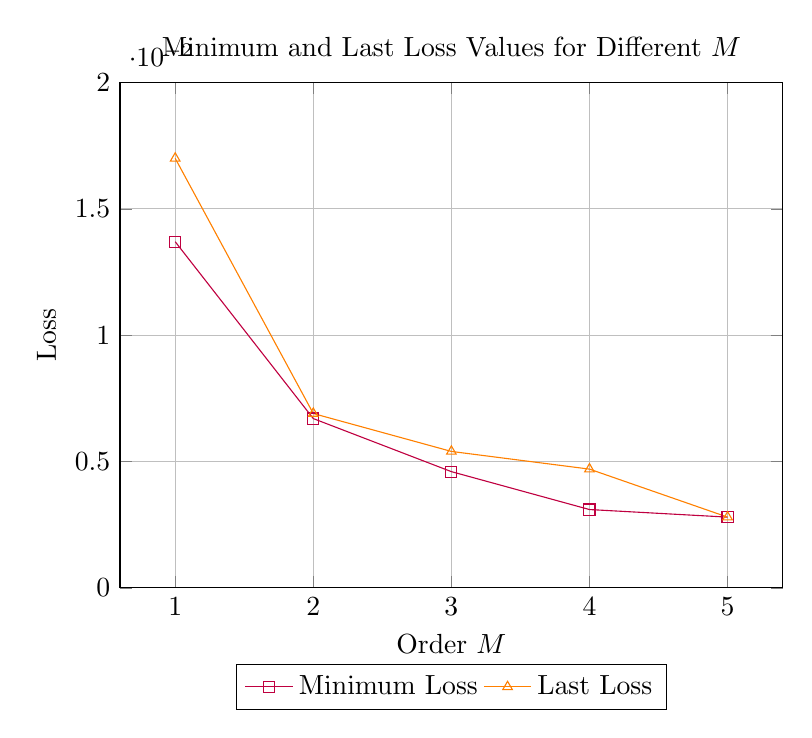
\begin{tikzpicture}
        \begin{axis}[
            width=10cm, height=8cm,
            xlabel={Order \( M \)},
            ylabel={Loss},
            xtick={1, 2, 3, 4, 5},
            legend style={at={(0.5,-0.15)}, anchor=north, legend columns=-1},
            ymin=0, ymax=0.02,
            grid=both,
            title={Minimum and Last Loss Values for Different \( M \)}
        ]
        % Minimum Loss
        \addplot[color=purple, mark=square] coordinates {
            (1, 0.0137)
            (2, 0.0067)
            (3, 0.0046)
            (4, 0.0031)
            (5, 0.0028)
        };
        \addlegendentry{Minimum Loss}

        % Last Loss
        \addplot[color=orange, mark=triangle] coordinates {
            (1, 0.0170)
            (2, 0.0069)
            (3, 0.0054)
            (4, 0.0047)
            (5, 0.0028)
        };
        \addlegendentry{Last Loss}
        \end{axis}
    \end{tikzpicture}
    \caption{Minimum and last loss values as a function of \( M \).}
    \label{fig:loss_M}
\end{figure}

\subsection{Error Analysis Varying \( M \)}

Figure \ref{fig:error_M} presents the errors in the \( x \), \( y \), and \( z \) directions for each value of \( M \). We observe a reduction in errors with increasing \( M \), particularly along the \( z \)-axis, suggesting that higher values of \( M \) contribute to a more accurate approximation of the solution, especially along certain dimensions.

\begin{figure}[h!]
    \centering
    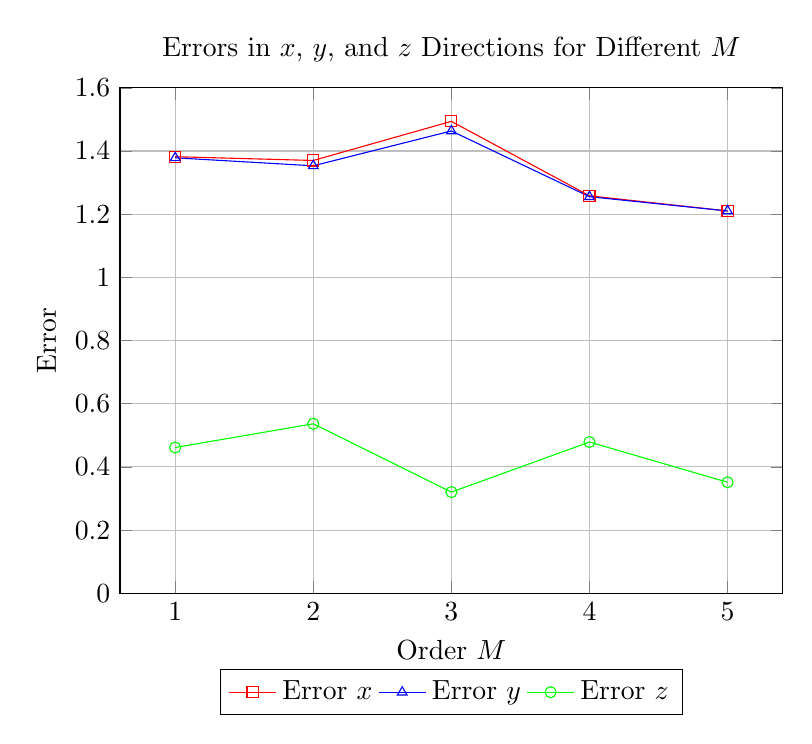
\begin{tikzpicture}
        \begin{axis}[
            width=10cm, height=8cm,
            xlabel={Order \( M \)},
            ylabel={Error},
            xtick={1, 2, 3, 4, 5},
            legend style={at={(0.5,-0.15)}, anchor=north, legend columns=-1},
            ymin=0, ymax=1.6,
            grid=both,
            title={Errors in \( x \), \( y \), and \( z \) Directions for Different \( M \)}
        ]
        % Error_x
        \addplot[color=red, mark=square] coordinates {
            (1, 1.3821)
            (2, 1.3702)
            (3, 1.4940)
            (4, 1.2583)
            (5, 1.2103)
        };
        \addlegendentry{Error \( x \)}

        % Error_y
        \addplot[color=blue, mark=triangle] coordinates {
            (1, 1.3786)
            (2, 1.3533)
            (3, 1.4636)
            (4, 1.2554)
            (5, 1.2103)
        };
        \addlegendentry{Error \( y \)}

        % Error_z
        \addplot[color=green, mark=o] coordinates {
            (1, 0.4615)
            (2, 0.5365)
            (3, 0.3203)
            (4, 0.4788)
            (5, 0.3514)
        };
        \addlegendentry{Error \( z \)}
        \end{axis}
    \end{tikzpicture}
    \caption{Errors along the \( x \), \( y \), and \( z \) directions as a function of \( M \).}
    \label{fig:error_M}
\end{figure}

\subsection{Summary of \( M \) Analysis}

From the above plots, it is evident that increasing \( M \) leads to a decrease in both the last loss and errors, with some variability across the \( x \), \( y \), and \( z \) components. These results suggest that optimizing the parameter \( M \) could play a critical role in improving the model's accuracy and efficiency in future applications.


\section{Comparison with Traditional Numerical Methods}

There exist many numerical methods, each useful in different situations. Each method has its own advantages and disadvantages, and its utility depends on the specific context and problem being addressed.

In general, numerical methods can be challenging to implement. They require complete knowledge of the system's parameters and usually work within simple domains. When studying dynamical systems, a numerical method may lose accuracy over long time periods, accumulating errors at each iteration. In contrast, a well-trained PINN could capture the system's behavior and provide a more accurate long-term solution.

While training a PINN can be costly in terms of time and computational resources, a properly trained PINN can generalize the system's dynamics and predict different solutions under varying parameters. This approach represents an innovative method that combines our understanding of neural networks with traditional numerical methods. Although it may not always achieve the same accuracy and can sometimes be more computationally expensive, its potential is remarkable.

\section{Conclusion}

In summary, increasing the number of neurons per layer generally reduces the error and minimum loss, indicating improved performance. However, the diminishing returns on errors along \( x \) and \( y \) suggest that further increases may not yield significant gains. The 80x5 configuration provides a good balance between accuracy and stability, while the 100x5 configuration shows signs of overfitting or instability, as indicated by the increased last loss. 

Similarly, increasing \( M \) results in lower errors and improved convergence, emphasizing its importance in optimizing the PINN for this system.


